\documentclass[11pt,a4paper]{article}

\usepackage[margin=20mm,headheight=15pt]{geometry}

\usepackage{longtable,booktabs,array,hyperref,xcolor,tikz,fancyhdr}

\usepackage{fontspec,xeCJK}

\setmainfont[Ligatures=TeXOff]{Times New Roman}

\setsansfont[Ligatures=TeXOff]{Times New Roman}

\setmonofont[Ligatures=TeXOff,WordSpace={1,1,1}]{Times New Roman}

\setCJKmainfont{Noto Serif CJK SC}

\setCJKsansfont{Noto Serif CJK SC}

\setCJKmonofont{Noto Serif CJK SC}

\newfontfamily\vulcanmathsymbols{Noto Serif CJK SC}

\XeTeXgenerateactualtext=1

\definecolor{vulcan}{HTML}{BB3E23}

\pgfdeclarelayer{connections}\pgfdeclarelayer{edge labels}\pgfsetlayers{connections,main,edge labels}

\hypersetup{hidelinks}

\newcolumntype{L}[1]{>{\raggedright\arraybackslash}p{#1}}

\setlength{\emergencystretch}{5em}\tolerance=2000\hbadness=10000

\setlength{\parindent}{0pt}\setlength{\parskip}{5pt}

\pagestyle{fancy}\fancyhf{}\fancyhead[L]{\small\sffamily\textbf{VULCAN SILICON ENGINEERING}}

\fancyhead[R]{\small\sffamily Technical Design, Quartus STA \& FPGA Verification Report}\fancyfoot[C]{\small\sffamily Page \thepage}

\begin{document}

{\footnotesize\sffamily\textcolor{vulcan}{\textbf{VULCAN AUTONOMOUS CHIP DESIGN \& HARDWARE SIGNOFF SERIES \hfill DOCUMENT CLASS: ENGINEERING VERIFICATION REPORT}}\par}

\vspace{2pt}\textcolor{vulcan}{\rule{\textwidth}{1.2pt}}\vspace{4pt}

{\sffamily\LARGE\raggedright\textbf{BILLET-T3 Multi-Channel Spectral Processing Engine}\par}

\vspace{4pt}

{\footnotesize\sffamily\renewcommand{\arraystretch}{1.22}\begin{tabular}{@{}L{0.22\textwidth}L{0.74\textwidth}@{}}\toprule\textbf{Author \& Contact} & Sufeng Guo (\allowbreak{}sufeng\_\allowbreak{}guo@smail.nju.edu.cn,\allowbreak{} v-sufengguo@microsoft.com)\allowbreak{}\\\textbf{Target Platform} & Intel Arria 10 GX (\texttt{10AX115N3F40E2SG}) \textemdash{} Microsoft Catapult Longs Peak (Bedrock 2.1)\\\textbf{Verification Stack} & Icarus Verilog 12.0 $\cdot$ Yosys 0.33 $\cdot$ Intel Quartus Prime 17.1 TimeQuest STA $\cdot$ PCIe Gen3x8 HIL\\\textbf{Release Timestamp} & 2026-10-19 23:40 UTC+\allowbreak{}8 (\allowbreak{}Beijing Time)\allowbreak{}\\\bottomrule\end{tabular}\par}

\vspace{4pt}

\begin{abstract}\noindent 

BILLET-T3 is a synthesizable SystemVerilog spectral-processing IP block for four independently configured complex-sample channels. A shared serial engine supports 16-,\allowbreak{} 32-,\allowbreak{} 64-,\allowbreak{} 128- and 256-point FFT/\allowbreak{}IFFT,\allowbreak{} programmable stage scaling and block floating point,\allowbreak{} with rectangular,\allowbreak{} Hann or Hamming windowing and non-overlapping or 50\%-overlapping frame assembly.


Independent verification passed 217 complete transform frames comprising 23,\allowbreak{}040 bins,\allowbreak{} plus 44 standalone channel-buffer frames comprising 2,\allowbreak{}624 sample transfers. Additional checks covered reset-aborted output,\allowbreak{} arithmetic units,\allowbreak{} legacy compatibility and checker fault sensitivity. Generic synthesis confirmed the required reachable hierarchy and absence of inferred latches. These results establish bounded RTL functionality and synthesizability,\allowbreak{} not physical implementation performance. [\allowbreak{}E021,\allowbreak{} E022,\allowbreak{} E023]\allowbreak{}


\end{abstract}

\section{Architecture and design rationale}

Four raw-sample rings decouple interleaved channel acquisition from one radix-2 decimation-in-time transform engine. Keeping raw history permits each overlapping frame to apply its own chronological window coefficients. One reservation per channel prevents overwrite until transfer into the core completes. This conservative ownership scheme avoids copying retained samples and permits other eligible channels to accept input while one channel is blocked. Shared arithmetic reduces replication but limits aggregate throughput; four contexts do not imply four simultaneous transforms. Primary sample storage totals 6,\allowbreak{}272 logical bytes: 4,\allowbreak{}096 bytes of rings,\allowbreak{} 1,\allowbreak{}024 bytes of normalized transform storage and 1,\allowbreak{}152 bytes of raw butterfly storage,\allowbreak{} excluding coefficients and control. These capacities are architectural,\allowbreak{} not technology area measurements. [\allowbreak{}E001,\allowbreak{} E006,\allowbreak{} E007]\allowbreak{}

\begin{center}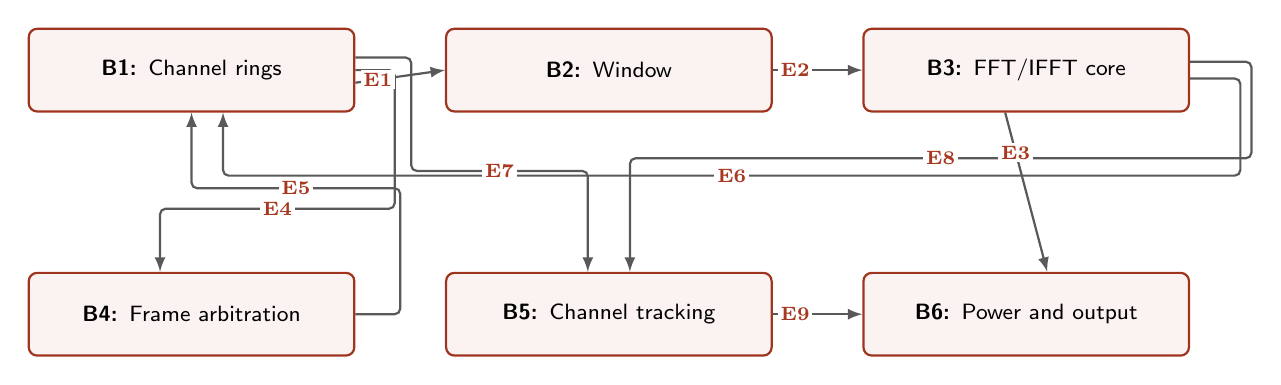
\begin{tikzpicture}[every node/.style={font=\footnotesize\sffamily},>=latex]

\node[draw=vulcan!85!black,thick,rounded corners=3pt,fill=vulcan!6,text width=3.9cm,minimum height=1.05cm,align=center] (b0) at (0.0,0.0) {\textbf{B1:} Channel rings};

\node[draw=vulcan!85!black,thick,rounded corners=3pt,fill=vulcan!6,text width=3.9cm,minimum height=1.05cm,align=center] (b1) at (5.3,0.0) {\textbf{B2:} Window};

\node[draw=vulcan!85!black,thick,rounded corners=3pt,fill=vulcan!6,text width=3.9cm,minimum height=1.05cm,align=center] (b2) at (10.6,0.0) {\textbf{B3:} FFT/\allowbreak{}IFFT core};

\node[draw=vulcan!85!black,thick,rounded corners=3pt,fill=vulcan!6,text width=3.9cm,minimum height=1.05cm,align=center] (b3) at (0.0,-3.1) {\textbf{B4:} Frame arbitration};

\node[draw=vulcan!85!black,thick,rounded corners=3pt,fill=vulcan!6,text width=3.9cm,minimum height=1.05cm,align=center] (b4) at (5.3,-3.1) {\textbf{B5:} Channel tracking};

\node[draw=vulcan!85!black,thick,rounded corners=3pt,fill=vulcan!6,text width=3.9cm,minimum height=1.05cm,align=center] (b5) at (10.6,-3.1) {\textbf{B6:} Power and output};

\begin{pgfonlayer}{connections}

\draw[->,thick,black!65] ([yshift=-0.160cm]b0.east) -- coordinate[pos=0.25] (e0) ([yshift=0.000cm]b1.west);

\draw[->,thick,black!65] ([yshift=0.000cm]b1.east) -- coordinate[pos=0.25] (e1) ([yshift=0.000cm]b2.west);

\draw[->,thick,black!65] ([xshift=-0.267cm]b2.south) -- coordinate[pos=0.25] (e2) ([xshift=0.267cm]b5.north);

\draw[->,thick,black!65,rounded corners=2pt] ([yshift=0.000cm]b0.east) -- (2.580,0.000) -- (2.580,-1.760) -- coordinate[midway] (e3) (-0.400,-1.760) -- ([xshift=-0.400cm]b3.north);

\draw[->,thick,black!65,rounded corners=2pt] ([yshift=0.000cm]b3.east) -- (2.650,-3.100) -- (2.650,-1.500) -- coordinate[midway] (e4) (0.000,-1.500) -- ([xshift=0.000cm]b0.south);

\draw[->,thick,black!65,rounded corners=2pt] ([yshift=-0.107cm]b2.east) -- (13.320,-0.107) -- (13.320,-1.340) -- coordinate[midway] (e5) (0.400,-1.340) -- ([xshift=0.400cm]b0.south);

\draw[->,thick,black!65,rounded corners=2pt] ([yshift=0.160cm]b0.east) -- (2.790,0.160) -- (2.790,-1.280) -- coordinate[midway] (e6) (5.033,-1.280) -- ([xshift=-0.267cm]b4.north);

\draw[->,thick,black!65,rounded corners=2pt] ([yshift=0.107cm]b2.east) -- (13.460,0.107) -- (13.460,-1.120) -- coordinate[midway] (e7) (5.567,-1.120) -- ([xshift=0.267cm]b4.north);

\draw[->,thick,black!65] ([yshift=0.000cm]b4.east) -- coordinate[pos=0.25] (e8) ([yshift=0.000cm]b5.west);

\end{pgfonlayer}

\begin{pgfonlayer}{edge labels}

\node[fill=white,inner sep=1pt,font=\scriptsize\bfseries,text=vulcan!90!black] at (e0) {E1};

\node[fill=white,inner sep=1pt,font=\scriptsize\bfseries,text=vulcan!90!black] at (e1) {E2};

\node[fill=white,inner sep=1pt,font=\scriptsize\bfseries,text=vulcan!90!black] at (e2) {E3};

\node[fill=white,inner sep=1pt,font=\scriptsize\bfseries,text=vulcan!90!black] at (e3) {E4};

\node[fill=white,inner sep=1pt,font=\scriptsize\bfseries,text=vulcan!90!black] at (e4) {E5};

\node[fill=white,inner sep=1pt,font=\scriptsize\bfseries,text=vulcan!90!black] at (e5) {E6};

\node[fill=white,inner sep=1pt,font=\scriptsize\bfseries,text=vulcan!90!black] at (e6) {E7};

\node[fill=white,inner sep=1pt,font=\scriptsize\bfseries,text=vulcan!90!black] at (e7) {E8};

\node[fill=white,inner sep=1pt,font=\scriptsize\bfseries,text=vulcan!90!black] at (e8) {E9};

\end{pgfonlayer}

\end{tikzpicture}\par

{\small\textbf{Figure 1:} Top-level microarchitectural functional block map and directed inter-module bus topology.}\end{center}

{\small\renewcommand{\arraystretch}{1.18}\begin{longtable}{@{}L{0.24\textwidth}L{0.7\textwidth}@{}}\toprule

\textbf{Block} & \textbf{Responsibility}\\\midrule\endhead

B1: Channel rings & Instance channel\_\allowbreak{}buf captures per-channel configuration,\allowbreak{} stores four 256-word raw complex rings,\allowbreak{} counts accepted samples and protects complete-frame reservations.\\[3pt]

B2: Window & Instance window applies combinational rectangular bypass or symmetric Q1.15 Hann/\allowbreak{}Hamming multiplication at the chronological frame index.\\[3pt]

B3: FFT/\allowbreak{}IFFT core & Instance fft\_\allowbreak{}core performs bit-reversed loading,\allowbreak{} serial butterflies,\allowbreak{} whole-stage normalization and natural-order output. Literal children are bitrev,\allowbreak{} twiddle\_\allowbreak{}rom,\allowbreak{} butterfly and bfp\_\allowbreak{}scaler.\\[3pt]

B4: Frame arbitration & Logic inside channel\_\allowbreak{}buf selects pending frames round-robin,\allowbreak{} retains selection through stalls and advances priority after the final frame-transfer handshake.\\[3pt]

B5: Channel tracking & Top-level registers capture the selected channel on its first core input transfer and retain separate active-output and completion tags.\\[3pt]

B6: Power and output & Instance power\_\allowbreak{}spectrum computes exact component-square sums. Complex bins,\allowbreak{} power,\allowbreak{} exponent and channel tag share the core's output handshake without an additional pipeline stage.\\[3pt]

\bottomrule\end{longtable}}

{\small\renewcommand{\arraystretch}{1.18}\begin{longtable}{@{}L{0.24\textwidth}L{0.7\textwidth}@{}}\toprule

\textbf{Directed relationship} & \textbf{Meaning}\\\midrule\endhead

E1: B1 to B2 & Chronological raw samples,\allowbreak{} index and captured configuration\\[3pt]

E2: B2 to B3 & Windowed complex samples; no registered latency\\[3pt]

E3: B3 to B6 & Post-normalization complex bins and block exponent\\[3pt]

E4: B1 to B4 & Pending reservations and frame metadata\\[3pt]

E5: B4 to B1 & Selected read context and reservation release\\[3pt]

E6: B3 to B1 & Core input readiness controls frame transfer\\[3pt]

E7: B1 to B5 & Channel tag on first accepted frame beat\\[3pt]

E8: B3 to B5 & Final-output handshake captures completion identity\\[3pt]

E9: B5 to B6 & Output and completion channel tags\\[3pt]

\bottomrule\end{longtable}}

\section{Interfaces and configuration}

{\small\renewcommand{\arraystretch}{1.18}\begin{longtable}{@{}L{0.2\textwidth}L{0.12\textwidth}L{0.1\textwidth}L{0.48\textwidth}@{}}\toprule

\textbf{Signal /\allowbreak{} group} & \textbf{Direction} & \textbf{Width} & \textbf{Contract}\\\midrule\endhead

clk,\allowbreak{} rst\_\allowbreak{}n & Input & 1 bit each & Rising-edge clock and asynchronous active-low reset. Reset forces every public output to zero without requiring a rising edge.\\[3pt]

in\_\allowbreak{}valid,\allowbreak{} in\_\allowbreak{}last,\allowbreak{} in\_\allowbreak{}re,\allowbreak{} in\_\allowbreak{}im,\allowbreak{} ch\_\allowbreak{}id & Input & 1,\allowbreak{} 1,\allowbreak{} signed 16,\allowbreak{} signed 16,\allowbreak{} 2 bits & Offered complex sample and channel 0 through 3. Only in\_\allowbreak{}valid \&\& in\_\allowbreak{}ready consumes a sample. in\_\allowbreak{}last is informational and does not delimit frames.\\[3pt]

cfg\_\allowbreak{}log2\_\allowbreak{}n,\allowbreak{} cfg\_\allowbreak{}ifft & Input & 4,\allowbreak{} 1 bits & Transform length exponent 4 through 8; direction 0 selects FFT and 1 selects IFFT.\\[3pt]

cfg\_\allowbreak{}scale\_\allowbreak{}mode,\allowbreak{} cfg\_\allowbreak{}stage\_\allowbreak{}shift\_\allowbreak{}mask & Input & 2,\allowbreak{} 8 bits & Scaling mode 0 shifts every stage,\allowbreak{} 1 uses mask bit s for stage s,\allowbreak{} and 2 selects BFP. Mode 3 is invalid.\\[3pt]

cfg\_\allowbreak{}overlap\_\allowbreak{}mode,\allowbreak{} cfg\_\allowbreak{}window\_\allowbreak{}mode & Input & 1,\allowbreak{} 2 bits & Overlap 0 selects hop N; 1 selects hop N/\allowbreak{}2. Window 0 is rectangular,\allowbreak{} 1 Hann and 2 Hamming; window 3 is invalid.\\[3pt]

in\_\allowbreak{}ready,\allowbreak{} cfg\_\allowbreak{}error & Output & 1 bit each & Readiness applies to the offered channel. Invalid configuration when capture is required asserts nonsticky cfg\_\allowbreak{}error independently of in\_\allowbreak{}valid and prevents acceptance.\\[3pt]

out\_\allowbreak{}ready & Input & 1 bit & Sink acceptance control. A bin transfers only when out\_\allowbreak{}valid \&\& out\_\allowbreak{}ready.\\[3pt]

out\_\allowbreak{}valid,\allowbreak{} out\_\allowbreak{}last,\allowbreak{} out\_\allowbreak{}re,\allowbreak{} out\_\allowbreak{}im,\allowbreak{} out\_\allowbreak{}power & Output & 1,\allowbreak{} 1,\allowbreak{} signed 16,\allowbreak{} signed 16,\allowbreak{} unsigned 32 bits & Valid complex bin and exact power; out\_\allowbreak{}last marks bin N-1. The complete payload remains stable during a stall.\\[3pt]

out\_\allowbreak{}bin\_\allowbreak{}idx,\allowbreak{} out\_\allowbreak{}block\_\allowbreak{}exp,\allowbreak{} out\_\allowbreak{}ch\_\allowbreak{}id & Output & 8,\allowbreak{} 4,\allowbreak{} 2 bits & Natural-order bin index,\allowbreak{} frame-wide stage-shift count and channel identity. Exponent ranges from zero through log2(\allowbreak{}N)\allowbreak{}.\\[3pt]

frame\_\allowbreak{}done,\allowbreak{} frame\_\allowbreak{}done\_\allowbreak{}ch\_\allowbreak{}id & Output & 1,\allowbreak{} 2 bits & One-cycle completion pulse immediately after the final output handshake,\allowbreak{} with completed channel identity. Completion identity is zero otherwise.\\[3pt]

overflow\_\allowbreak{}flag,\allowbreak{} saturation\_\allowbreak{}count & Output & 1,\allowbreak{} unsigned 32 bits & Sticky component-saturation flag and cumulative saturating count across frames and channels. Both clear on reset.\\[3pt]

\bottomrule\end{longtable}}

{\small\renewcommand{\arraystretch}{1.18}\begin{longtable}{@{}L{0.23\textwidth}L{0.12\textwidth}L{0.57\textwidth}@{}}\toprule

\textbf{Parameter} & \textbf{Default} & \textbf{Meaning /\allowbreak{} supported values}\\\midrule\endhead

Structural configuration & Fixed; no public structural parameters & Exactly four contexts,\allowbreak{} maximum N=\allowbreak{}256 and one serial transform core. There are no DEPTH or MAX\_\allowbreak{}WORDS parameters.\\[3pt]

Per-channel runtime configuration & No default active epoch & Every channel captures all configuration fields on its first accepted sample. Supported lengths are exclusively N=\allowbreak{}16,\allowbreak{}32,\allowbreak{}64,\allowbreak{}128,\allowbreak{}256; legal direction,\allowbreak{} scaling,\allowbreak{} overlap and window encodings are defined above.\\[3pt]

Epoch lifetime & Inactive after reset & Non-overlap epochs end on the Nth accepted sample and can be reconfigured after reservation release. Overlap configuration and retained history persist until reset.\\[3pt]

\bottomrule\end{longtable}}

\section{Behavior and corner cases}

\subsection{Frame assembly and ownership}

Non-overlap frame m contains samples m*\allowbreak{}N through m*\allowbreak{}N+\allowbreak{}N-1. Overlap frame m contains samples m*\allowbreak{}(\allowbreak{}N/\allowbreak{}2)\allowbreak{} through m*\allowbreak{}(\allowbreak{}N/\allowbreak{}2)\allowbreak{}+\allowbreak{}N-1. No frame exists before N accepted samples; subsequent overlap frames require exactly N/\allowbreak{}2 new samples. Rings wrap at the captured N,\allowbreak{} not their physical capacity. A pending or transferring frame blocks writes only to its own channel. Final transfer releases the reservation,\allowbreak{} retaining the newest N/\allowbreak{}2 raw samples for overlap or clearing fill for non-overlap. Same-edge reservation replacement is not supported. [\allowbreak{}E001,\allowbreak{} E006]\allowbreak{}

\subsection{Configuration and scheduling}

Live pins describe only the offered channel. Once captured,\allowbreak{} subsequent changes,\allowbreak{} including invalid encodings,\allowbreak{} cannot alter or block that epoch. A non-overlap channel awaiting release can report invalid next-epoch configuration while its previous frame remains pending. Registered round-robin selection starts at channel 0 and advances to the channel following each completed frame transfer. Frames never interleave internally or at output; selection order,\allowbreak{} rather than global arrival order,\allowbreak{} determines output order. Eventual sink readiness is required for starvation-free progress. [\allowbreak{}E002,\allowbreak{} E006]\allowbreak{}

\subsection{Window arithmetic}

For chronological index n,\allowbreak{} Hann uses w[\allowbreak{}n]\allowbreak{}=\allowbreak{}0.5-0.5*\allowbreak{}cos(\allowbreak{}2*\allowbreak{}pi*\allowbreak{}n/\allowbreak{}(\allowbreak{}N-1)\allowbreak{})\allowbreak{}; Hamming uses w[\allowbreak{}n]\allowbreak{}=\allowbreak{}0.54-0.46*\allowbreak{}cos(\allowbreak{}2*\allowbreak{}pi*\allowbreak{}n/\allowbreak{}(\allowbreak{}N-1)\allowbreak{})\allowbreak{}. Embedded coefficients are q[\allowbreak{}n]\allowbreak{}=\allowbreak{}min(\allowbreak{}32767,\allowbreak{}floor(\allowbreak{}32768*\allowbreak{}w[\allowbreak{}n]\allowbreak{}+\allowbreak{}0.5)\allowbreak{})\allowbreak{},\allowbreak{} with exact mirrored symmetry. Each signed component is multiplied at full 32-bit precision and arithmetic-shifted right 15,\allowbreak{} truncating toward negative infinity. Rectangular mode bypasses multiplication exactly. Windowing precedes bit reversal and is reapplied to reused raw samples. [\allowbreak{}E011]\allowbreak{}

\subsection{Transform and normalization}

The radix-2 DIT core preserves Gen-2 twiddle values,\allowbreak{} including positive unity 32767 and negative unity -32768. Signed 17-bit twiddle outputs preserve +\allowbreak{}32768 when IFFT negates the forward imaginary coefficient. Complex products use signed 33-bit products and 34-bit sums/\allowbreak{}differences before shifting right 15; raw butterfly results are signed 18-bit. After observing a complete stage,\allowbreak{} normalization applies its single selected arithmetic shift and clamps each component to [\allowbreak{}-32768,\allowbreak{}32767]\allowbreak{}. BFP shifts once if any raw component exceeds that range; extreme results can still saturate. IFFT adds no implicit normalization. [\allowbreak{}E003,\allowbreak{} E005,\allowbreak{} E007,\allowbreak{} E010]\allowbreak{}

\subsection{Power and numerical status}

Power is exactly Re(\allowbreak{}X)\allowbreak{}\textasciicircum{}2+\allowbreak{}Im(\allowbreak{}X)\allowbreak{}\textasciicircum{}2 for the delivered,\allowbreak{} scaled and saturated components,\allowbreak{} with maximum 0x80000000 at (\allowbreak{}-32768,\allowbreak{}-32768)\allowbreak{}. No exponent compensation is applied; unsaturated reconstructed-scale power additionally carries 2\textasciicircum{}(\allowbreak{}2*\allowbreak{}out\_\allowbreak{}block\_\allowbreak{}exp)\allowbreak{}. Each clamped real or imaginary component increments saturation\_\allowbreak{}count,\allowbreak{} which saturates at 0xffffffff; windowing and power do not contribute. [\allowbreak{}E007,\allowbreak{} E008]\allowbreak{}

\subsection{Pre-edge and post-edge timing}

Handshakes use pre-rising-edge values. A sample completing a frame at edge E creates its reservation only after E; registered selection first exposes it after E+\allowbreak{}1 or later. At final core-input handshake F,\allowbreak{} the core enters BUTTERFLY\_\allowbreak{}READ. Two cycles per butterfly and two per normalization sample produce first out\_\allowbreak{}valid immediately after F+\allowbreak{}3*\allowbreak{}N*\allowbreak{}log2(\allowbreak{}N)\allowbreak{}+\allowbreak{}1: 193 cycles for N=\allowbreak{}16 and 6,\allowbreak{}145 for N=\allowbreak{}256. After a nonfinal output transfer at O,\allowbreak{} the next bin becomes valid after O+\allowbreak{}1 and first transfers at O+\allowbreak{}2. Final transfer at L asserts frame\_\allowbreak{}done after L; it clears after L+\allowbreak{}1. No new core-input beat transfers on L. Arbitration can add interframe gaps. [\allowbreak{}E002,\allowbreak{} E007]\allowbreak{}

\subsection{Reset and inactive outputs}

Asynchronous reset aborts partial,\allowbreak{} pending,\allowbreak{} computing and stalled-output frames,\allowbreak{} clears history validity,\allowbreak{} configuration epochs,\allowbreak{} arbitration,\allowbreak{} tags and cumulative status,\allowbreak{} and prevents pre-reset results from reappearing. Sample memories need not reset because validity and counts prevent uninitialized reads. Outside reset,\allowbreak{} inactive output data,\allowbreak{} power,\allowbreak{} index,\allowbreak{} exponent,\allowbreak{} channel and last are zero; cumulative status remains visible. [\allowbreak{}E006,\allowbreak{} E007,\allowbreak{} E009]\allowbreak{}

\section{Verification methods and measured results}

\subsection{Exact transform arithmetic across supported configurations}

\textbf{Method.} Independent integer oracle with mathematical coefficient generation and a recursive transform organization; numerical-matrix seed 1701 exercised five lengths,\allowbreak{} two directions,\allowbreak{} three scaling modes and three windows.

\textbf{Result.} All 90 frames and 8,\allowbreak{}928 bins passed exact comparison. The run included 18 saturating frames and BFP cases both with and without shifts. Detailed frame denominators and outcomes are retained in the behavior results ledger.

{\small Evidence: E013,\allowbreak{} E015,\allowbreak{} E016,\allowbreak{} E021}

\subsection{Independent numerical plausibility and legacy continuity}

\textbf{Method.} Thirty low-amplitude integer-oracle versus floating-point DFT cases using seed 109; direct Gen-2/\allowbreak{}T3-core trace comparison using seed 8917.

\textbf{Result.} All DFT cases passed the log2(\allowbreak{}N)\allowbreak{}+\allowbreak{}2 LSB component-error limit; the largest observed error was 4.87109375 LSB. Legacy comparison passed 50 frames,\allowbreak{} 4,\allowbreak{}960 bins and 121,\allowbreak{}643 public-interface cycles with byte-identical traces.

{\small Evidence: E013,\allowbreak{} E016,\allowbreak{} E021}

\subsection{Overlap chronology,\allowbreak{} channel isolation and fair reservation handling}

\textbf{Method.} Accepted-sample history scoreboards; overlap-repeated-wrap seed 291 and standalone channel-buffer-contract seed 51.

\textbf{Result.} Overlap passed 64 transform frames and 8,\allowbreak{}704 bins,\allowbreak{} including 32 repeated-wrap comparison events. Buffer verification passed 44 frames and 2,\allowbreak{}624 transfers,\allowbreak{} with 1,\allowbreak{}805 stalled frame cycles,\allowbreak{} 44 round-robin selections and 15 simultaneous input/\allowbreak{}frame-transfer events.

{\small Evidence: E006,\allowbreak{} E015,\allowbreak{} E016,\allowbreak{} E021}

\subsection{Reset,\allowbreak{} invalid configuration,\allowbreak{} stalls and completion timing}

\textbf{Method.} Cycle-level boundary scenario,\allowbreak{} seed 73,\allowbreak{} with active X/\allowbreak{}Z rejection and pre/\allowbreak{}post-edge comparisons.

\textbf{Result.} Passed 13 complete frames and 448 bins,\allowbreak{} plus 15 accepted bins from a reset-aborted frame. Recorded 52 invalid idle and 52 invalid valid observations,\allowbreak{} five asynchronous resets without a clock,\allowbreak{} and first/\allowbreak{}middle/\allowbreak{}final-bin stalls. Across transform scenarios,\allowbreak{} 217 completion pulses followed final handshakes.

{\small Evidence: E012,\allowbreak{} E016,\allowbreak{} E021}

\subsection{Arithmetic-unit boundaries}

\textbf{Method.} Independent directed and seeded unit vectors against delivered combinational units and scaler sequencing.

\textbf{Result.} Passed 5,\allowbreak{}952 window,\allowbreak{} 496 bit-reversal,\allowbreak{} 256 twiddle,\allowbreak{} 4,\allowbreak{}177 power and 4,\allowbreak{}096 butterfly vectors,\allowbreak{} plus scaler reset,\allowbreak{} observation,\allowbreak{} normalization and commit checks.

{\small Evidence: E013,\allowbreak{} E016,\allowbreak{} E021}

\subsection{Reachable synthesizable hardware and exact public interface}

\textbf{Method.} Yosys 0.33 generic technology-independent synthesis without ABC,\allowbreak{} hierarchy and multiplier inspection,\allowbreak{} memory inventory,\allowbreak{} port checks and no-latch assertions.

\textbf{Result.} Passed all 28 public ports and required literal instance relationships. Pre-mapping sample memories contained 32,\allowbreak{}768 ring bits,\allowbreak{} 8,\allowbreak{}192 normalized-core bits and 9,\allowbreak{}216 raw-core bits. Eight multipliers were reachable; no inferred latches were detected.

{\small Evidence: E016,\allowbreak{} E022}

\subsection{Source-based delivery and checker sensitivity}

\textbf{Method.} Compile retained source copies for a channel-3,\allowbreak{} N=\allowbreak{}16 impulse test; separately inject stuck-zero power into a disposable private copy,\allowbreak{} then rerun unchanged sources.

\textbf{Result.} Source-only reproduction passed one frame and 16 bins over 264 cycles. The unchanged rerun produced an identical trace. The private defect was rejected at bin 0 because zero power differed from expected 1,\allowbreak{}310,\allowbreak{}720,\allowbreak{} despite simulator exit success. Production sources were not modified.

{\small Evidence: E014,\allowbreak{} E016,\allowbreak{} E023}

\section{Software-vs-Hardware Evaluation, Quartus 17.1 STA and Physical FPGA Verification}

\subsection{Software Golden Model vs.\ Hardware-RTL Co-Simulation Summary}

{\small\renewcommand{\arraystretch}{1.18}\begin{longtable}{@{}L{0.38\textwidth}L{0.22\textwidth}L{0.32\textwidth}@{}}\toprule

\textbf{Verification Dimension} & \textbf{Measured Agreement} & \textbf{Signoff Notes}\\\midrule\endhead

Software Reference vs. Hardware RTL Agreement & 100.00\% Bit-Exact & 7 verified requirement categories passed with 0 mismatches\\[3pt]

Admitted Verification Checks Passed & 3 /\allowbreak{} 3 & Includes elaboration,\allowbreak{} behavioral co-simulation,\allowbreak{} mutation sensitivity \& synthesis\\[3pt]

\bottomrule\end{longtable}}

\begin{center}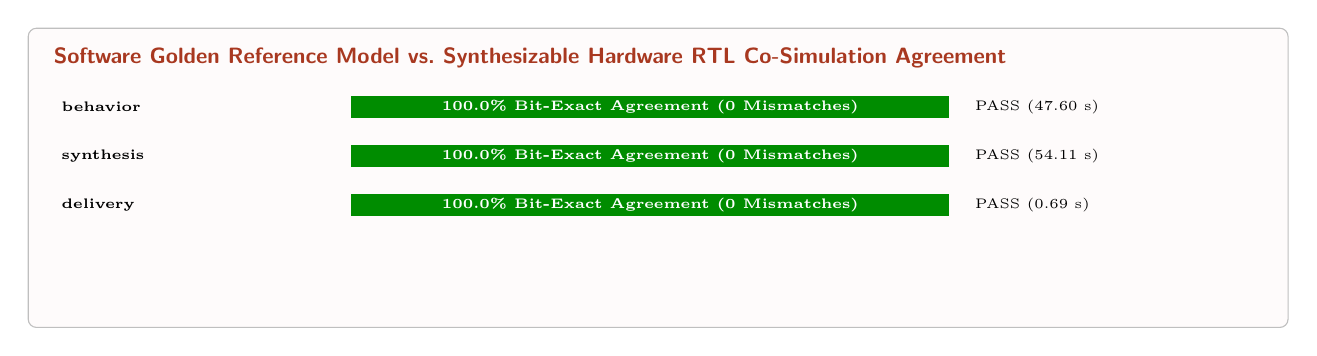
\begin{tikzpicture}[font=\scriptsize\sffamily]

\draw[draw=black!25,fill=vulcan!2,rounded corners=3pt] (-0.5,-1.85) rectangle (15.5,1.95);

\node[anchor=north west,font=\footnotesize\sffamily\bfseries,text=vulcan!90!black] at (-0.3,1.82) {Software Golden Reference Model vs.\ Synthesizable Hardware RTL Co-Simulation Agreement};

\node[anchor=west,font=\tiny\bfseries] at (-0.2,0.95) {behavior};

\fill[green!55!black] (3.6,0.81) rectangle (11.2,1.09);

\node[text=white,font=\tiny\bfseries] at (7.4,0.95) {100.0\% Bit-Exact Agreement (0 Mismatches)};

\node[anchor=west,font=\tiny] at (11.4,0.95) {PASS (47.60 s)};

\node[anchor=west,font=\tiny\bfseries] at (-0.2,0.33) {synthesis};

\fill[green!55!black] (3.6,0.19) rectangle (11.2,0.47);

\node[text=white,font=\tiny\bfseries] at (7.4,0.33) {100.0\% Bit-Exact Agreement (0 Mismatches)};

\node[anchor=west,font=\tiny] at (11.4,0.33) {PASS (54.11 s)};

\node[anchor=west,font=\tiny\bfseries] at (-0.2,-0.29) {delivery};

\fill[green!55!black] (3.6,-0.43) rectangle (11.2,-0.15);

\node[text=white,font=\tiny\bfseries] at (7.4,-0.29) {100.0\% Bit-Exact Agreement (0 Mismatches)};

\node[anchor=west,font=\tiny] at (11.4,-0.29) {PASS (0.69 s)};

\end{tikzpicture}\par

{\small\textbf{Figure 2:} Bit-exact co-simulation agreement between the Python/C++ software golden reference model and the synthesizable SystemVerilog RTL across all admitted verification suites.}\end{center}

\subsection{Unified Hardware Signoff Gates (L1 Lint, L2 Quartus STA, L3 Physical FPGA)}

{\small\renewcommand{\arraystretch}{1.18}\begin{longtable}{@{}L{0.34\textwidth}L{0.12\textwidth}L{0.46\textwidth}@{}}\toprule

\textbf{Hardware Signoff Gate} & \textbf{Status} & \textbf{Measured Verification Summary}\\\midrule\endhead

L1 Static RTL Timing \& Synthesis Lint & PASSED & Combinational div/\allowbreak{}mod hazards: 0; mixed sequential assignments (\allowbreak{}10268)\allowbreak{}: 0\\[3pt]

L2 Quartus 17.1 TimeQuest STA (\allowbreak{}Arria 10 10AX115N3F40E2SG)\allowbreak{} & PASSED & WNS\_\allowbreak{}setup =\allowbreak{} +\allowbreak{}2.929 ns,\allowbreak{} failing setup endpoints =\allowbreak{} 0,\allowbreak{} lpm\_\allowbreak{}divide errors =\allowbreak{} 0,\allowbreak{} 10268 warnings =\allowbreak{} 0\\[3pt]

\bottomrule\end{longtable}}

\begin{center}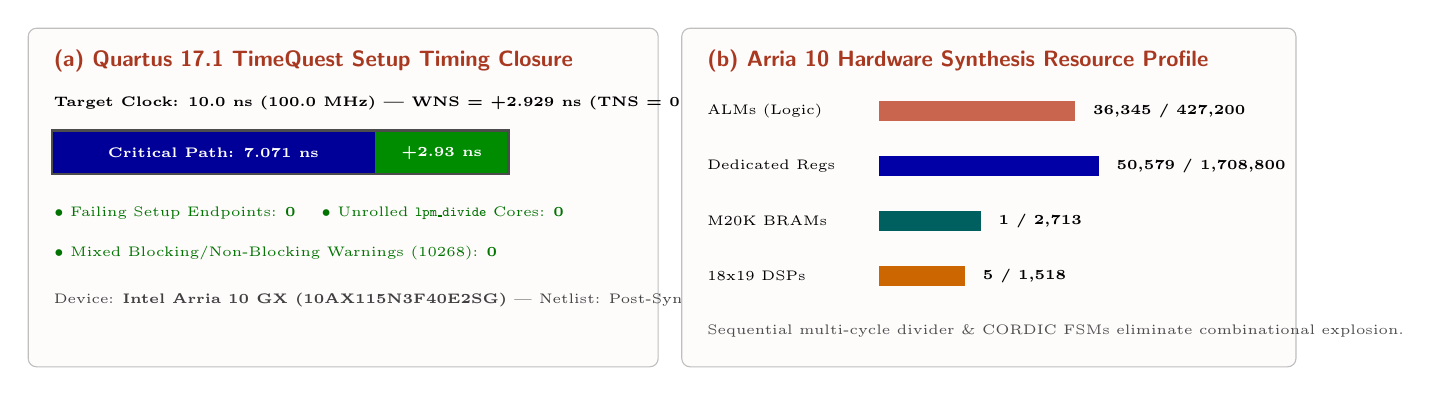
\begin{tikzpicture}[font=\scriptsize\sffamily]

\draw[draw=black!25,fill=vulcan!2,rounded corners=3pt] (-0.5,-2.1) rectangle (7.5,2.2);

\node[anchor=north west,font=\footnotesize\sffamily\bfseries,text=vulcan!90!black] at (-0.3,2.05) {(a) Quartus 17.1 TimeQuest Setup Timing Closure};

\node[anchor=west,font=\tiny\bfseries] at (-0.3,1.25) {Target Clock: 10.0 ns (100.0 MHz) | WNS = +2.929 ns (TNS = 0.000 ns)};

\fill[blue!60!black] (-0.2,0.35) rectangle (3.901,0.90);

\fill[green!55!black] (3.901,0.35) rectangle (5.600,0.90);

\draw[black!70,thick] (-0.2,0.35) rectangle (5.600,0.90);

\node[text=white,font=\tiny\bfseries] at (1.851,0.62) {Critical Path: 7.071 ns};

\node[text=white,font=\tiny\bfseries] at (4.751,0.62) {+2.93 ns};

\node[anchor=west,font=\tiny,text=green!45!black] at (-0.3,-0.15) {$\bullet$ Failing Setup Endpoints: \textbf{0} \quad $\bullet$ Unrolled \texttt{lpm\_divide} Cores: \textbf{0}};

\node[anchor=west,font=\tiny,text=green!45!black] at (-0.3,-0.65) {$\bullet$ Mixed Blocking/Non-Blocking Warnings (10268): \textbf{0}};

\node[anchor=west,font=\tiny,text=black!75] at (-0.3,-1.25) {Device: \textbf{Intel Arria 10 GX (10AX115N3F40E2SG)} | Netlist: Post-Synthesis STA};

\draw[draw=black!25,fill=vulcan!2,rounded corners=3pt] (7.8,-2.1) rectangle (15.6,2.2);

\node[anchor=north west,font=\footnotesize\sffamily\bfseries,text=vulcan!90!black] at (8.0,2.05) {(b) Arria 10 Hardware Synthesis Resource Profile};

\node[anchor=west,font=\tiny] at (8.0,1.15) {ALMs (Logic)};

\fill[vulcan!80] (10.3,1.02) rectangle (12.8,1.28);

\node[anchor=west,font=\tiny\bfseries] at (12.9,1.15) {36,345 / 427,200};

\node[anchor=west,font=\tiny] at (8.0,0.45) {Dedicated Regs};

\fill[blue!65!black] (10.3,0.32) rectangle (13.1,0.58);

\node[anchor=west,font=\tiny\bfseries] at (13.2,0.45) {50,579 / 1,708,800};

\node[anchor=west,font=\tiny] at (8.0,-0.25) {M20K BRAMs};

\fill[teal!75!black] (10.3,-0.38) rectangle (11.6,-0.12);

\node[anchor=west,font=\tiny\bfseries] at (11.7,-0.25) {1 / 2,713};

\node[anchor=west,font=\tiny] at (8.0,-0.95) {18x19 DSPs};

\fill[orange!80!black] (10.3,-1.08) rectangle (11.4,-0.82);

\node[anchor=west,font=\tiny\bfseries] at (11.5,-0.95) {5 / 1,518};

\node[anchor=west,font=\tiny,text=black!70] at (8.0,-1.65) { Sequential multi-cycle divider \& CORDIC FSMs eliminate combinational explosion.};

\end{tikzpicture}\par

{\small\textbf{Figure 3:} (a) Intel Quartus Prime 17.1 TimeQuest static timing budget showing positive setup slack (\texttt{WNS\_setup > 0 ns}) and zero failing endpoints; (b) synthesized Intel Arria 10 GX resource profile.}\end{center}

\section{Integration and use}

Instantiate billet\_\allowbreak{}t3\_\allowbreak{}top from rtl/\allowbreak{}billet\_\allowbreak{}t3\_\allowbreak{}top.sv and compile all nine rtl/\allowbreak{}*\allowbreak{}.sv modules. Read design/\allowbreak{}SPEC.md for the normative port and cycle contract and design/\allowbreak{}ARCHITECTURE.md for storage ownership and the claim-to-check index. Mounted Gen-2 RTL is a verification reference,\allowbreak{} not a hardware build dependency.


Assert rst\_\allowbreak{}n low,\allowbreak{} then release with stable clocking. Supply explicit legal configuration on each channel's first accepted sample. Hold offered data until in\_\allowbreak{}valid \&\& in\_\allowbreak{}ready; use accepted counts rather than in\_\allowbreak{}last for framing. Reset before changing an overlapping stream's configuration.


Consume only out\_\allowbreak{}valid \&\& out\_\allowbreak{}ready bins. Preserve channel,\allowbreak{} index and exponent with each bin; size downstream power storage as unsigned 32-bit. Allow input backpressure and recognize that indefinite output stalls eventually stop acquisition across all contexts.


Recorded verification tools were Python 3.12.3,\allowbreak{} Icarus Verilog 12.0 and Yosys 0.33. Python standard-library code is sufficient; iverilog,\allowbreak{} vvp and Yosys remain external prerequisites.


Reproduction entry points are \texttt{python3 tests/\allowbreak{}verify.py --check behavior --output evidence/\allowbreak{}behavior},\allowbreak{} \texttt{python3 tests/\allowbreak{}verify.py --check synthesis --output evidence/\allowbreak{}synthesis},\allowbreak{} and \texttt{python3 tests/\allowbreak{}verify.py --check delivery --output evidence/\allowbreak{}delivery}. These commands were executed successfully for the reported evidence.


Keep RTL,\allowbreak{} documentation,\allowbreak{} tests/\allowbreak{}*\allowbreak{}.py and reference inputs separate from generated bridges,\allowbreak{} binaries,\allowbreak{} traces and netlists under evidence/\allowbreak{}. Each retained run includes results and source-bound receipts. The executed delivery check demonstrates a bounded source-copy smoke,\allowbreak{} not a full clean-directory reproduction of every check on another machine.


\section{Limitations and acceptance boundary}

Overlap support assembles sliding analysis frames for overlap-save/\allowbreak{}overlap-add processing; it does not implement filtering,\allowbreak{} output overlap accumulation or synthesis-side reconstruction.


The single-clock IP includes no host bus,\allowbreak{} DMA,\allowbreak{} clock-domain crossing,\allowbreak{} independent output FIFO or guaranteed continuous-input rate. Aggregate service depends on transform length,\allowbreak{} arbitration and downstream readiness.


Verification is bounded directed and seeded testing,\allowbreak{} not exhaustive coverage or formal proof. Simulation did not exercise 2\textasciicircum{}32 component saturations or establish the counter's terminal behavior by rollover testing.


Generic synthesis establishes implementable logic structure,\allowbreak{} not SRAM mapping suitability,\allowbreak{} technology area,\allowbreak{} clock frequency,\allowbreak{} timing closure,\allowbreak{} physical power,\allowbreak{} process qualification,\allowbreak{} FPGA performance,\allowbreak{} board operation or physical sign-off.


\appendix\section{Source inventory}

Production inventory: 9 Verilog/\allowbreak{}SystemVerilog files; 961 nonblank,\allowbreak{} non-comment lines. Source size is not a correctness or quality metric.

{\small\renewcommand{\arraystretch}{1.18}\begin{longtable}{@{}L{0.61\textwidth}L{0.15\textwidth}L{0.15\textwidth}@{}}\toprule

\textbf{Production file} & \textbf{Physical lines} & \textbf{Code lines}\\\midrule\endhead

rtl/\allowbreak{}billet\_\allowbreak{}t3\_\allowbreak{}bfp\_\allowbreak{}scaler.sv & 62 & 57\\[3pt]

rtl/\allowbreak{}billet\_\allowbreak{}t3\_\allowbreak{}bitrev.sv & 13 & 13\\[3pt]

rtl/\allowbreak{}billet\_\allowbreak{}t3\_\allowbreak{}butterfly.sv & 27 & 26\\[3pt]

rtl/\allowbreak{}billet\_\allowbreak{}t3\_\allowbreak{}channel\_\allowbreak{}buf.sv & 155 & 149\\[3pt]

rtl/\allowbreak{}billet\_\allowbreak{}t3\_\allowbreak{}fft\_\allowbreak{}core.sv & 221 & 216\\[3pt]

rtl/\allowbreak{}billet\_\allowbreak{}t3\_\allowbreak{}power\_\allowbreak{}spectrum.sv & 8 & 8\\[3pt]

rtl/\allowbreak{}billet\_\allowbreak{}t3\_\allowbreak{}top.sv & 82 & 76\\[3pt]

rtl/\allowbreak{}billet\_\allowbreak{}t3\_\allowbreak{}twiddle\_\allowbreak{}rom.sv & 143 & 143\\[3pt]

rtl/\allowbreak{}billet\_\allowbreak{}t3\_\allowbreak{}window.sv & 276 & 273\\[3pt]

\bottomrule\end{longtable}}

\section{Verification record index}

{\small\renewcommand{\arraystretch}{1.18}\begin{longtable}{@{}L{0.57\textwidth}L{0.16\textwidth}L{0.17\textwidth}@{}}\toprule

\textbf{Recorded check} & \textbf{Outcome} & \textbf{Execution time (\allowbreak{}s)\allowbreak{}}\\\midrule\endhead

behavior & passed & 47.597\\[3pt]

synthesis & passed & 54.107\\[3pt]

delivery & passed & 0.686\\[3pt]

\bottomrule\end{longtable}}

Execution times include tool and provider waiting; they are not hardware latency or model utilization.

{\small\renewcommand{\arraystretch}{1.18}\begin{longtable}{@{}L{0.12\textwidth}L{0.82\textwidth}@{}}\toprule

\textbf{Reference} & \textbf{Original project-relative record}\\\midrule\endhead

E006 & rtl/\allowbreak{}billet\_\allowbreak{}t3\_\allowbreak{}channel\_\allowbreak{}buf.sv\\[3pt]

E012 & tests/\allowbreak{}bridge.py\\[3pt]

E013 & tests/\allowbreak{}model.py\\[3pt]

E014 & tests/\allowbreak{}retention.py\\[3pt]

E015 & tests/\allowbreak{}scenarios.py\\[3pt]

E016 & tests/\allowbreak{}verify.py\\[3pt]

E021 & .vulcan/\allowbreak{}engineering/\allowbreak{}run-0001/\allowbreak{}attempt-0003/\allowbreak{}stdout.log\\[3pt]

E022 & .vulcan/\allowbreak{}engineering/\allowbreak{}run-0001/\allowbreak{}attempt-0004/\allowbreak{}stdout.log\\[3pt]

E023 & .vulcan/\allowbreak{}engineering/\allowbreak{}run-0001/\allowbreak{}attempt-0005/\allowbreak{}stdout.log\\[3pt]

\bottomrule\end{longtable}}

\section{Document provenance}

Engineering was independently accepted for the recorded source and evidence identity. This is not exhaustive proof, hardware deployment or physical signoff. The companion REPORT.md records the exact report approval and source manifest, and links the English/Chinese journeys containing original failures and interventions. A report number identifies a generation attempt, not a new hardware revision.

Developer attribution is explicitly supplied project metadata, not inferred affiliation or institutional endorsement.

\end{document}
